\begin{figure}[t]
    \centering
    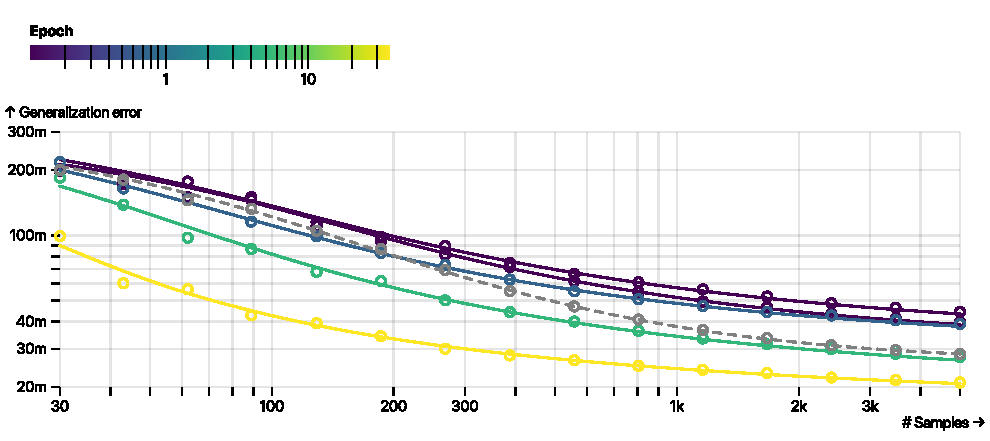
\includegraphics[scale=0.6]{chapters/deeprf/figs/art_opt_emp1.pdf}
    \caption{
    Test error when training the readout layer only of a relu-activated three-layer neural network during training, using the \texttt{Tensorflow} implementation of the Adam \cite{kingma2014adam} optimizer, over $120$ epochs with batch size $128$. (dashed): ridge regression. The data is sampled from a Gaussian distribution with mean and variance matching the distribution of MNIST images. In all training procedures, the regularization parameter has been numerically optimized. Solid lines represent the theoretical prediction of Theorem \ref{thm genRMT informal}, dots represent numerical experiments. For more details we refer to~\Cref{synth MNIST}. 
    }
    \label{fig:inductive_bias}
\end{figure}


The previous discussion addressed feature maps associated to random Gaussian networks. However, note that the linearization itself only involves products of the weights matrices, and coefficient depending on weight covariances which can straightforwardly be estimated therefrom. The linearization \ref{def: linearized_covs} can thus be readily heuristically evaluated  for feature maps associated to deterministic \textit{trained} finite-width neural networks. As we discuss later in this section, the resulting prediction for the test error captures well the learning curves when re-training the readout weights of the network in a number settings. Naturally, such settings correspond to lazy learning regimes \cite{Jacot2020}, where the network feature map is effectively \textit{linear}, thus little expressive. However, these trained feature map, albeit linear, can still encode some inductive bias, as shown by \cite{Ba2022} for one gradient step in the shallow case. In this section, we briefly explore these questions for fully trained deep networks, through the lens of our theoretical results.

Fig.\,\ref{fig:inductive_bias} contrasts the test error achieved by linear regression (red), and regression on the feature map associated to a three-layer student at initialization (green) and after $3000$ epochs of end-to-end training using full-batch Adam \cite{kingma2014adam} at learning rate $10^{-4}$ and weight decay $10^{-3}$ over $n_0=1400$ training samples (blue). For all curves, the readout weights were trained using ridge regression, with regularization strength optimized over using cross-validation. Solid curves indicate the theoretical predictions of Thm. \ref{thm genRMT informal} leveraging the closed-form linearized formulae \ref{def: linearized_covs} for the features covariance. Interestingly, even for the deterministic trained network features, the formula captures the learning curve well. This observation temptingly suggests to interpret the feature map $\f(x)$ as the stochastic linear map
\begin{align}
 \label{eq: effective_linear_net}
 \f^g(x)=W_{\mathrm{eff.}}x+C_{\mathrm{eff.}}^{\frac{1}{2}}\xi
\end{align}
where $W_{\mathrm{eff.}}\in\R^{p\times d}$ is proportional to the product of all the weight matrices
\begin{align}
    W_{\mathrm{eff.}}=\left(\prod\limits_{\ell=1}^L \kappa^1_\ell\right) \hat{W}_L\hat{W}_{L-1}\dots \hat{W}_1 
\end{align}
and $\xi\sim\mathcal{N}(0,\mathbb{I}_p)$ is a stochastic noise colored by the covariance
\begin{align}
    \label{eq:effective_cov}
    C_{\mathrm{eff.}}\equiv & \sum\limits_{\ell=1}^{L-1}
    \left(\kappa^*_\ell\prod\limits_{s=\ell+1}^L
    \kappa_s^1
    \right)^2  \hat{W}_L\dots \hat{W}_{\ell+1}\hat{W}_{\ell+1}^\top\dots \hat{W}_L^\top\notag \\
                    & +  (\kappa^*_L)^2\mathbb{I}_{p_L}.
\end{align}
Note that the effective linear network \eqref{eq: effective_linear_net} simply corresponds to the composition of the equivalent stochastic linear layers \eqref{eq:linearized-layer}. A very similar expression for the covariance of the effective structured noise \eqref{eq:effective_cov} appeared in \cite{schroder2023deterministic} for the random case with unstructured and untrained random weights. The effective linear model \eqref{eq: effective_linear_net} affords a concise viewpoint on a deep finite-width non-linear network trained in the lazy regime. On an intuitive level, during training, the network effectively tunes the two matrices $W_{\mathrm{eff.}},C_{\mathrm{eff.}}$ which parametrize the effective model \eqref{eq: effective_linear_net}. Indeed, the interplay between these two matrices -- both depending on the weights $\hat{W}_{\ell}$ -- defines the inductive bias of the trained network in the high-dimensional regime, which ultimately determines the generalization properties of the network. To see this explicitly, consider the ridge regression problem on the effective linear features in \cref{eq: effective_linear_net}. Changing variables $\beta = \frac{C_{\mathrm{eff.}}^{\frac{1}{2}}\theta}{\sqrt{p}}$ and assuming for simplicity that $C_{\mathrm{eff.}}$ is invertible, this yields the following effective problem:\looseness=-1
\begin{align}
    \label{eq:def:erm_equiv}
    \underset{\beta\in\R^{\p}}{\min}~&\sum\limits_{i\in[\n]}\left(\y_{i}-\beta^\top(C_{\mathrm{eff.}}^{-\frac{1}{2}}W_{\mathrm{eff.}}\x_{i}+\xi_i)\right)^{2}\!\! +p\lambda\beta^{\top}C^{-1}_{\mathrm{eff.}}\beta.\notag
\end{align}
In this basis, the effective linear features has two components: an irreducible isotropic noise $\xi_{i}$ and a term $C^{-\frac{1}{2}}_{\mathrm{eff.}}W_{\mathrm{eff.}}\x_{i}$ controlling the (linear) representation of the training data. A key difference with respect to the deep unstructured case of \cite{schroder2023deterministic} is that the effective $\ell_2$-regularization is anisotropic.

For a (typically employed) random isotropic initialization, the initial network is equivalent to a unstructured dRF. In particular, the unstructured dRF inductive bias \cite{Jacot2020} is not aligned to the target, treating all directions equally. In terms of generalization, since the effective linear features are noisy, this implies that the initial generalization error is lower-bounded by the best ridge estimator \cite{schroder2023deterministic}. As the network is trained, the weights $\hat{W}_{\ell}$ adapt to the target, implying that even in the regime where the linearization in \cref{eq: effective_linear_net} holds, the effective linear problem \cref{eq: effective_linear_net} can regularize different directions adaptively, potentially outperforming the ridge regression baseline. The fact that the optimal regularization for ridge regression on linear feature maps might be anisotropic has been explored in detail in \cite{Wu2020OnTO}.\looseness=-1 

 
The learning of beneficial inductive biases over training is illustrated by Fig.\,\ref{fig:inductive_bias} for synthetic data. Despite the fact that all represented feature maps are effectively just linear feature maps, they can still encode very different biases, yielding different phenomenology. In particular, remark that, when trained over a sufficient number of epochs, the trained feature map outperforms by ridge regression on the whole range of probed sample complexities -- suggesting the trained weights $W_{\mathrm{eff.}},C_{\mathrm{eff.}}$ learned some form of helpful inductive bias, and allow for a more performant linear model. A similar qualitative behaviour can also be observed in real data sets, as illustrated in Fig.\ref{fig:real_MNIST}.


\begin{figure}
    \centering
    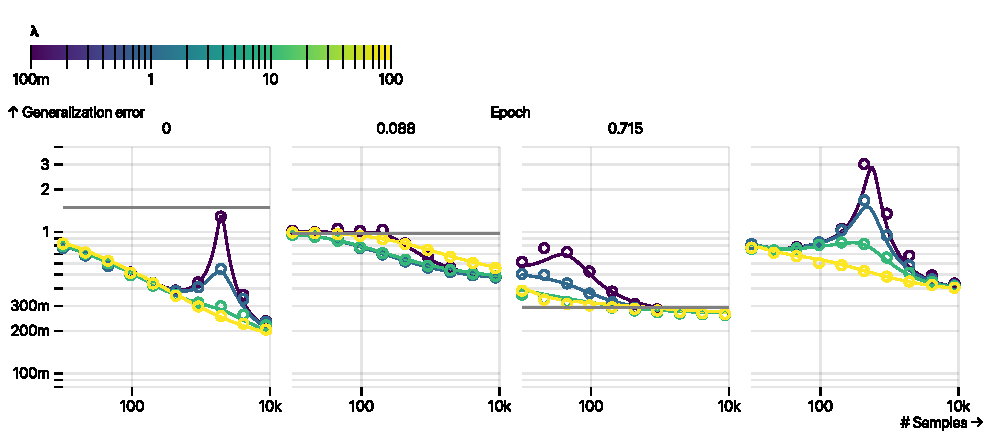
\includegraphics[scale=0.6]{chapters/deeprf/figs/real_emp_660.pdf}
    \caption{Test error when re-training the readout layer only of an Adam-optimized relu-activated three-layer neural network, trained on a regression task on MNIST. Labels are $+1$ (resp. $-1$) for even (resp. odd) digits. Solid lines represent the theoretical prediction of Theorem \ref{thm genRMT informal}, dots represent numerical experiments on the real dataset. Different colors indicate different reguarization strengths $\lambda$. Different panels correspond to different training times. All details are provided in App.~\ref{app:real_data}.}
    \label{fig:real_MNIST}
\end{figure}

\section{Concluding remarks}
\paragraph{Real data ---}We observe that the theoretical predictions of Theorem \ref{thm genRMT informal} also capture the learning curves of trained networks on some \textit{real} datasets, when retraining the readout only using ridge regression, provided the features covariances $\Omega,\Phi,\Psi$ are estimated from data. Fig.\,\ref{fig:real_MNIST} contrasts the theoretical characterization of Theorem \ref{thm genRMT informal} with numerical experiments on MNIST \cite{lecun1998gradient}, for a three-neural network optimized with Adam \cite{kingma2014adam}, revealing overall good agreement. All experimental details are reported in Appendix \ref{app:real_data}. Note that closely related observations have also been made in \cite{Loureiro2021CapturingTL}.

\paragraph{Limitations ---} Our results provides an insight in the inductive bias of trained deep rainbow networks. However, as discussed in \cite{guth2023rainbow}, this only captures a subset of neural networks. Understanding the boundaries of applicability of the Gaussian rainbow framework (and hence of our theory) is an interesting problem. A recent line of work investigating the properties of two-layer neural networks after a single step of training \cite{Ba2022, dandi2023twolayer, moniri2024theory, cui2024asymptotics} provides a first clue. These works show that with an aggressive learning rate the hidden-layer weights can be approximated by a spiked random matrix model. Investigating under which conditions the asymptotic performance is equivalent to a structured Gaussian model is an interesting venue for future research. A similar problem was studied in the context of structured inputs in \cite{pesce23a, Gerace2024}.